% !TEX program = xelatex
\documentclass[a4paper]{ctexrep}

\usepackage{soul}
% \newcommand{\mod}[1]{{\color{red} #1}} %teal青色, magenta水红, violet紫
\newcommand{\yu}[1]{{\color{red} [ZY: #1]}} %teal青色, magenta水红, violet紫

\usepackage{import}
\usepackage{authblk}
\usepackage{booktabs}
\usepackage{longtable}
\usepackage{graphicx}
\usepackage{amssymb}
\usepackage{amsmath}
\usepackage{algorithmicx}
\usepackage{algpseudocode}
\usepackage[top=1in, bottom=1in, left=1.25in, right=1.25in]{geometry}

\usepackage{hyperref}
\hypersetup{
  colorlinks   = true, %Colours links instead of ugly boxes
  urlcolor     = cyan, %Colour for external hyperlinks
  linkcolor    = blue, %Colour of internal links
  citecolor    = red   %Colour of citations
}

\def\equationautorefname{式}%
\def\footnoteautorefname{脚注}%
\def\itemautorefname{项}%
\def\figureautorefname{图}%
\def\tableautorefname{表}%
\def\partautorefname{篇}%
\def\appendixautorefname{附录}%
\def\chapterautorefname{章}%
\def\sectionautorefname{节}%
\def\subsectionautorefname{小节}%
\def\subsubsectionautorefname{小小节}%
\def\paragraphautorefname{段落}%
\def\subparagraphautorefname{子段落}%
\def\FancyVerbLineautorefname{行}%
\def\theoremautorefname{定理}%

\usepackage{listings}
\lstset{
	keywordstyle	= blue,
	basicstyle		= \footnotesize\ttfamily,
	tabsize			  = 2,
	numbers			  = left,
	breaklines		= true,
	frame			    = tb
}

\pagestyle{plain}

\begin{document}

\title{
NASAC 2018 软件原型竞赛 \\
~~\\
\bf 违反编码规范的缺陷检测
}

\author{{\bf 参赛队员}: 张宇翔\thanks{Email: zyx504@mail.ustc.edu.cn}、邓胜亮、李森\\}
\author{{\bf 指导教师}:张昱\thanks{Email: yuzhang@ustc.edu.cn}}
\affil{中国科学技术大学,计算机科学与技术学院}

\maketitle
\tableofcontents
\newpage

\renewcommand\thesection{\arabic{section}}
\section{工具简介}
\label{sec:intro}
``违反编码规范的缺陷检测工具''(以下简称本工具)是根据NASAC2018软件原型命题竞赛组 
2018年10月21日晚发布的竞赛题目,
由中国科学技术大学计算机科学与技术学院张昱老师于10月22日
联络2018级硕士研究生张宇翔组队研制。
本参赛队由队长张宇翔、2016级本科生邓胜亮(10月23日加入)、
2018级硕士研究生李森(10月26日加入)组成,
工具研发的起止时间为2018年10月22日至11月10日;
张昱老师进行全程指导。

本参赛队利用 \href{https://clang.llvm.org/}{Clang 7.0.0} 
提供的工具框架
设计实现了具有可配置、易扩展的自动化违反编码规范的缺陷检测工具。
该工具提供函数参数合法性检查、函数错误返回码处理检查、
变量按需初始化检查、头文件自包含检查、循环依赖检查、
函数头注释检查、标识符命名检查等,
产生的诊断信息内容全面、可读性强。
用户可以方便地配置工具的行为,扩展其功能。

\subsection{功能简介}
\label{sec:intro:func}
该工具能够进行的检查如下:

\begin{itemize}
\item {\bf 函数参数合法性检查}
检查代码中模块对外接口是否进行了合法性检查。

\item{\bf 函数错误返回码处理检查}
检查在调用提供了错误指示机制的函数后,是否立即检查了错误指示。

\item{\bf 变量按需初始化检查}
检查代码中是否存在冗余的初始化。

\item{\bf 头文件自包含及循环包含检查}
检查头文件是否自包含且没有循环依赖。

\item{\bf 函数头注释检查}
检查函数头注释风格是否一致、注释中是否只有格式没有内容、是否说明了必要的信息、未注释的函数是否需要补充注释。

\item{\bf 标识符命名检查}
指出函数、变量名中的非英文单词,并对英文变量名提供常见的缩写建议。
\end{itemize}

所有检查的结果在汇报时都会指出其在源码中对应的位置(包括文件路径、行号、列号),方便用户进行修改。
各功能具体的实现细节将在 \S\ref{sec:core} 进行介绍。

\subsection{使用说明简介}
\label{sec:intro:usage}

该工具为命令行工具,用户通过提供命令行参数,对工具进行以下配置:

\begin{itemize}
    \item 关闭指定的一个或多个检查;
    \item 指定英文词典、缩写词典的位置;
    \item 指定返回错误码的函数列表的位置;
    \item 指定要检查的项目的编译命令列表位置;
    \item 指定要检查的文件或目录;
\end{itemize}

除了提供命令行选项以外,用户可以自行删减、扩充英文词典、缩写词典、返回错误码的函数列表,
从而方便地根据实际需要来定制工具的行为。

关于以上配置方式的具体说明见 \S\ref{sec:usage} 一节。

\section{技术核心}
\label{sec:core}

\subsection{整体架构}
\label{sec:core:arch}

\begin{figure}[htbp]
\centering
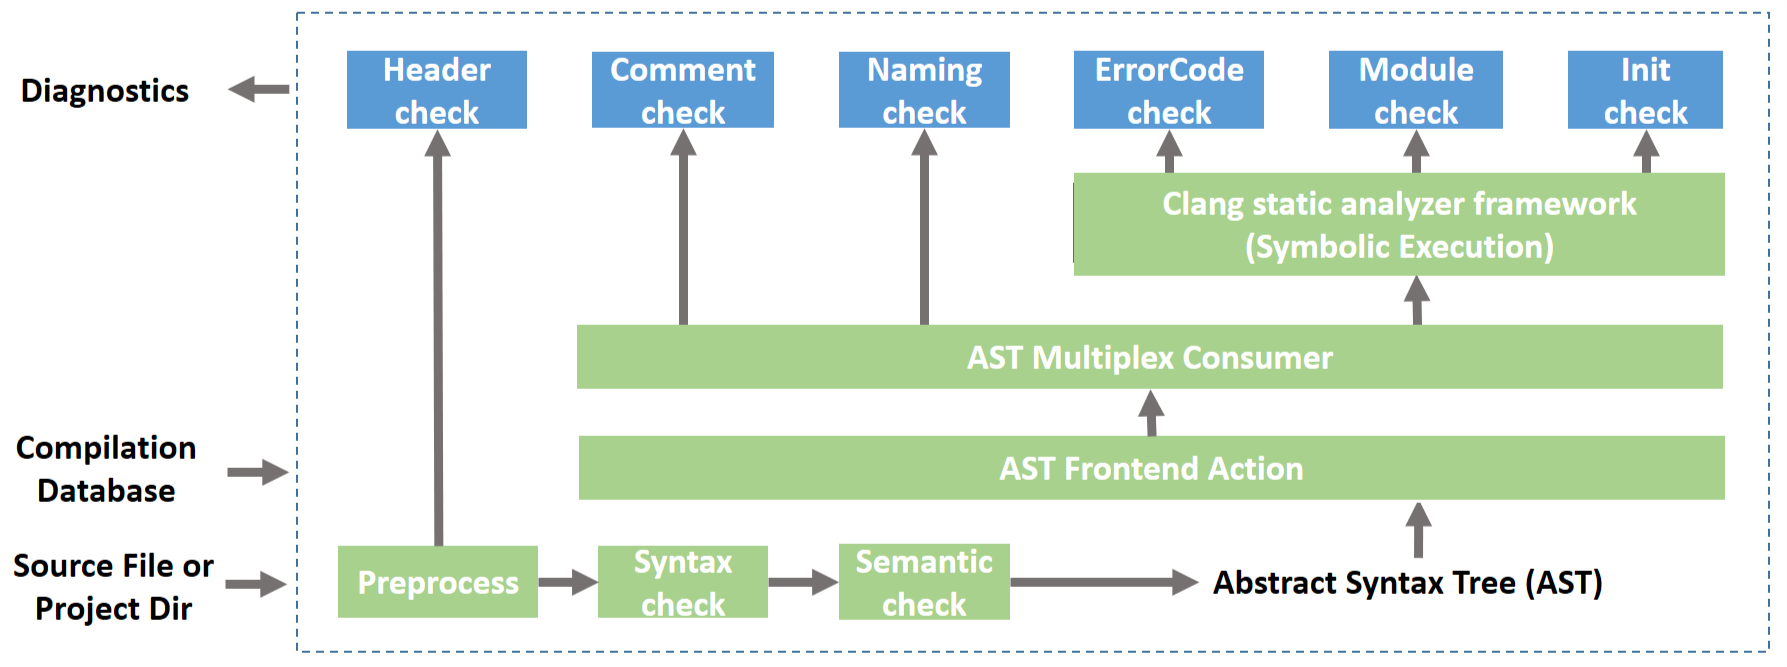
\includegraphics[width=\textwidth]{figure/architecture}
\caption{工具整体架构图}
\label{fig:arch}
\end{figure}

本工具整体基于\href{https://clang.llvm.org/}{Clang}框架扩展实现。
\autoref{fig:arch}展示了本工具的软件架构,
它接收待检查的源文件或项目目录与编译源文件使用的{\bf 编译命令数据库}(可选)作为输入,
检测和识别源文件中存在的违反编码规范的潜在缺陷,最后输出相应的诊断信息。
当输入为项目目录时,工具会递归地收集目录下所有的源文件依次处理。
\autoref{fig:arch}中以矩形色块表示对数据的操作,
绿色底色的矩形属于Clang框架提供的编译分析基础设施,
蓝色底色的矩形属于根据竞赛六点需求在Clang提供的基础设施上研制的相应检查。

输入工具的C程序文件会依次经历预处理、
语法检查和语义检查最终生成抽象语法树
(Abstract Syntax Tree, 简称AST)。
竞赛需求中有关头文件的相关检查(Header Check)
在预处理阶段通过\textbf{预处理器回调机制}实现;
其余五点需求通过AST结构上的一个前端动作(Frontend Action)的\textbf{多路AST消费者}来实现。
在五点需求中,
函数头注释检查(Comment Check)和命名检查(Naming Check)
直接实现为\href{https://clang.llvm.org/doxygen/classclang_1_1ASTConsumer.html}{ASTConsumer}子类,
而函数错误处理检查(ErrorCode Check)、模块内外调用规范检查(Module Check)
和按需初始化检查(Init Check)则
使用\href{https://clang-analyzer.llvm.org/}{Clang静态分析框架}进行\textbf{基于符号执行的路径敏感的过程内分析}。
针对输入的每个源文件和一条可能的编译命令,
工具只会对该源文件解析一次,六项检查会在这一次解析过程中依次完成。

后续六节会依次介绍各点需求实现策略,
\S\ref{sec:core:header}介绍需求一“头文件应当自包含,且没有循环依赖”的实现;
\S\ref{sec:core:arg}介绍需求二“模块内部函数参数的合法性检查,由调用者负责”的实现;
\S\ref{sec:core:error}介绍需求三“对函数的错误返回码要全面处理”的实现;
\S\ref{sec:core:naming}介绍需求四“除了常见的、通用缩写外,不使用单词缩写,不得使用汉语拼音”的实现;
\S\ref{sec:core:comment}介绍需求五“函数命名无法表达的信息,必须加函数头注释辅助说明”的实现;
\S\ref{sec:core:init}介绍需求六“变量或内存块,按需初始化;禁止冗余清零”的实现。

\subsection{头文件检查}
\label{sec:core:header}

\subsubsection{头文件自包含检查}

如果一个头文件是自包含的,
那么单独以该头文件作为本工具输入应正常通过预处理、语法检查和语义检查
生成合法的AST结构;
否则说明该头文件可能存在对未定义结构的引用,即不是自包含的。
本工具针对该项检查并不需要进行额外的定义,
而只需要基于Clang提供的基本编译流程即可判断。

\subsubsection{头文件循环包含检查}

头文件循环引用检查将头文件间的引用关系维护为有向图$G=\{V,E\}$,
其中顶点集合$V$中的元素表示头文件,
有向边集合$E$中的元素表示头文件间的包含关系,
通过检查最终图$G$是否有环判断头文件是否循环包含。

头文件循环包含检查的实现是基于Clang的预处理器回调对象(\href{https://clang.llvm.org/doxygen/classclang_1_1PPCallbacks.html}{PPCallback})来定制的,
主要关注回调事件列表中的
头文件包含事件(\href{https://clang.llvm.org/doxygen/classclang_1_1PPCallbacks.html#ad5509ca394c21faaead91ec8add75dd2}{InclusionDirective})和主文件结束事件(\href{https://clang.llvm.org/doxygen/classclang_1_1PPCallbacks.html#a63e170d069e99bc1c9c7ea0f3bed8bcc}{EndOfMainFile})。
本工具在头文件包含事件回调函数中记录
当前发起包含的文件绝对路径$u$和被包含的文件绝对路径$v$,
将$u$和$v$加入顶点集合$V$,将$(u,v)$加入有向边集合$E$。
本工具在主文件(作为工具输入的头文件)结束事件回调函数中检测图$G$
是否有环存在。
如果存在,则将构成环的头文件节点通过诊断引擎输出。

\subsection{函数参数合法性检查}
\label{sec:core:arg}

该项检查针对竞赛要求第二点进行实现,本参赛队对第二点的需求理解为:
考虑编译单元$U$ (一个C 程序文件为一个编译单元)中的函数$F$,
当$F$向编译单元外暴露时,即$F$未被 $static$ 修饰,
需要检查 $F$ 的输入参数的合法性;
否则,不需要检查 $F$ 的输入参数的合法性。
当 $F$ 调用函数 $G$ 时,如果 $G$ 与 $F$ 都在同一个编译单元 $U$ 中且不对外暴露,
那么 $G$ 参数的合法性将由 $F$ 负责检查,
否则 $F$ 不需要保证 $G$ 调用参数的合法性检查。

在上述理解中,“检查”针对的对象是内存区域存储的右值。
若内存区域的右值直接作为分支条件表达式的操作数,
那么就认为相应内存区域的右值得到检查。

本工具基于{\bf 不信任传播}的思想实现上述需求。
首先,根据需求设置某些内存区域右值为不信任源,
如需要检查的函数形参右值;
然后,
由不信任的右值经运算后导出的其他右值也不被信任。
当不信任的右值被读取时,本工具将产生警告;
当程序代码有对不信任的内存区域右值的“检查”,
则该右值获得信任,并且该右值定值时所依赖的所有内存区域右值也获得信任。


本工具采用Clang提供的静态分析框架对输入的源C 程序文件进行
基于符号执行的路径敏感的过程内分析。
在分析中,追踪的程序点状态定义如\autoref{equ:module_check_state}所示。
其中$S_1$表示内存区域右值(Memory Region Values, 简记RV)的信任状态,
$T$表示信任,$U$表示不信任;
$S_2$表示内存区域右值到最近一次定值时依赖的内存区域右值集合。
% 前者主要是为了在读取内存区域右值是判断是否右值检查过,
% 后者的目的主要是为了支持间接检查的情况,
% 典型的情况如需要错误处理的函数调用,
% 当函数调用返回的错误指示尚未检查前,该函数岀参可能存在错误,被认为处于未检查状态;
% 当错误指示检查后,认为函数岀参相应的处于已检查状态。

\begin{equation}
\label{equ:module_check_state}
S = \{
S_1 : RVs \mapsto \{T, U\}, 
S_2 : RVs \mapsto \{RVs\}
\}
\end{equation}

在上述程序状态基础上,
定义如\autoref{fig:module_check} 所示的转换规则和检查动作,
其中函数$Value()$接收一个左值并返回对应右值,
函数 $DependentRegionValues()$ 接收一个表达式 $E$
并返回 $E$ 中直接依赖的内存区域右值。
\begin{figure}[p]
\begin{tabular}{l}
$[[Entry]]: $\\
$\qquad S_1 = \phi, S_2=\phi; $\\
$[[ParmDecl\ X]]: $\\
$\qquad S_1[Value(X) \mapsto IsStatic(Func)\ ?\ T : U]; $\\
$[[VarDecl\ X]]: $\\
$\qquad S_1[Value(X) \mapsto U]; $\\
$[[Condition\ E]]: $\\
$\qquad \forall RV \in DependentRegionValues(E), S_1[RV \mapsto T]; $\\
$\qquad \forall RV' \in S_2(RV), S_1[RV' \mapsto T]; $\\
$Pre.[[E(E_1,E_2,...,E_n)]]: $\\
$\qquad \text{if}\ IsNotExtern(E),$\\
$\qquad \text{then} \forall E_i \in \{E_1,E_2,...,E_n\} \land S_1(E_i) = U,
\text{report unchecked argument}\ E_i; $\\
$Post.[[E(E_1,E_2,...,E_n)]]: $\\
$\qquad \text{if}\ NeedHandleError(E), $\\
$\qquad \text{then}\ \forall E_i \in \{E_1,E_2,...,E_n\} \land IsOutput(E, E_i), S_1[Value(E_i) \mapsto U]; $\\
$\qquad S_2[Value(E(E_1,E_2,...,E_n)) \mapsto DependentRegionValues(E(E_1,E_2,...,E_n))] $\\
$[[E_1 = E_2]]: $\\
$\qquad S_1[Value(E_1) \mapsto \forall RV \in DependentRegionValues(E), S_1(RV) = T\ ?\ T : U]; $\\
$\qquad S_2[Value(E_1) \mapsto DependentRegionValues(E_2)] $\\
$[[Read\ E]]: $\\
$\qquad \text{if}\ S_1(Value(E)) = U,\text{then report read before check};$
\end{tabular}
\caption{函数参数合法性检查状态转移与检查动作} \label{fig:module_check} 
\end{figure}


\subsection{错误处理检测}
\label{sec:core:error}
该检测主要对带有错误返回值的函数进行检查。
由于并非所有的函数都带有错误返回值,
所以首先应该筛选出带有错误返回值的函数。
例如,标准库中的文件操作函数(fopen,fclose等)就属于此类。

本工具对需要检查的函数\(f\)的错误返回值检查方法如下:

\begin{itemize}
  \item
    对于单独出现的函数调用\(f\),
在其出现位置后的第一条语句应当立即对函数返回值进行检查,且为条件判断,
而不应当再调用其他的函数,否则给出警告。
  \item
    如果函数调用 \(f\)直接出现在条件语句中,
则判断为一种直接检查,不给出警告。

\end{itemize}

由于不同函数的返回值未知,
并且不同函数(第三方函数/用户自定义函数)的返回值所表现出来的意义不同,
所以无法准确判断对当前函数调用是否需要进行返回值检查。
为此,本参赛队引入一个配置文件名为funcName.txt,用于存放带有错误返回值函数的函数名,包括标准库中常用的带有错误返回的函数。
一旦在运行程序中出现的函数名与当前文件中的记录相吻合时,
就断定该函数带有错误返回值,并立即对其进行检查。
本工具允许用户自行扩充包含错误返回值的第三方函数和用户自定义函数的名字列表。
 

\subsection{命名检测}
\label{sec:core:naming}

本工具对用户定义或声明的函数和变量的名称(标识符)进行检查。
对于每个标识符,
首先使用正则表达式 \texttt{{[}a-z{]}+\textbar{}{[}A-Z{]}{[}a-z{]}*} 
得到常见命名风格中的单词
(例如 message\_buffer、messageBuffer、MessageBuffer 这三种形式)。

接下来对于每个单词检查其中的缩写是否合法:
1) 如果该单词非英文单词且非领域常用缩写,则给出警告;
2) 如果该单词是变量名的一部分且存在常用缩写,则给出缩写建议。

本工具只对变量名给出缩写建议,
原因是我们认为通常函数名应当包含更全面、准确的含义,故不推荐过多使用缩写。

本工具使用从\url{https://github.com/dwyl/english-words}获得的英文单词词典,
其格式为每行一个单词,在比较时忽略大小写。
用户可对其自行扩充和替换。
该词典含有英文单词及其单复数等形式,因此可以避免大多数误报。

参考比赛要求和编程经验,本参赛队编写了一个简短的常用缩写词典,
其格式为``原始单词:缩写''。
用户可根据需要自行对其扩充和替换。

\subsection{函数头注释检测}
\label{sec:core:comment}

在 Clang 提供的框架下,调用

  \ \ \ \ \href{https://clang.llvm.org/doxygen/classclang_1_1ASTContext.html#ac10b2ebc25da948d370e74f7688fd134}{ASTContext::getRawCommentForDeclNoCache()} 
\\即可获取函数的头注释内容。

在获得函数的头注释后,本工具进行如下的检查:

\begin{itemize}
  \item
  检查注释风格(“/**/”、“//”之一)是否与之前出现的注释风格一致,如果不一致则汇报这一情况,并且不再对其他函数头注释进行检查以减少分析所耗时间。

  \item 
  如果函数存在指针类型的参数,则在注释中寻找该参数名(严格匹配)。
  如果找到则认为用户已经对该指针相关的内存约定做了说明,否则提示需要对该参数进行说明。

  \item 
  如果函数返回指针类型的变量,则在注释中寻找“返回”字样。
  如果找到,则认为用户已经对返回值做了说明,否则提示需要对返回值做说明。

  \item
  在注释中寻找后跟空白的冒号(正则表达式 \texttt{(:\textbar{}:)(\textbackslash{}\textbackslash{}s+\textbar{}\$)})。
  如果找到,则认为存在空有格式的注释,产生提示。

\end{itemize}

在仔细考虑竞赛题目要求后,本参赛队发现:检查在注释中是否说明性能约束、算法实现、可重入性是很难判断的,如处理不当,很容易导致大量误报。
为此,本参赛队没有实现相关的功能,但是用户可以根据实际需求,
在本工具设计和实现的 FullCommentChecker 类中添加相关的代码方便地扩充功能。

\subsection{按需初始化检测}
\label{sec:core:init}

按需初始化检测本质上关注的是避免对内存区域的冗余写操作,
即,如果对一内存区域的连续两次访问操作均为写操作,
那么前一次写操作就是冗余的。

本工具采用基于符号执行的路径敏感的过程内分析完成该类检测。
在分析过程中,本工具追踪的程序点状态定义如\autoref{equ:init_state}所示,
意为各内存区域(Memory Region,简记$MR$)的上一次访问操作类型,
$R$ 表示读操作,$W$ 表示写操作。

\begin{equation}
\label{equ:init_state}
S : MRs \mapsto \{ R, W \}
\end{equation}

在上述程序状态基础上,转换规则和检查动作定义如\autoref{fig:init_check} 所示。
其中函数 $Value()$ 接收一个左值并返回对应右值。

\begin{figure}[htbp]
\begin{tabular}{l}
$[[entry]]:$\\
$\qquad S = \phi;$\\
$[[read\ Region]]:$\\
$\qquad S[Region \mapsto R];$\\
$[[write\ Region]]:$\\
$\qquad \text{if}\ S(Region)=W,\text{then report reduntant write}; S[Region\mapsto W];$\\
$Post.[[E(E_1,E_2,...,E_n)]]:$\\
$\qquad \forall E_i \in \{E_1,E_2,...,E_n\} \land IsLValue(E_i),
S[Value(E_i) \mapsto IsOutput(E, E_i)\ ?\ W : R]$
\end{tabular}
\caption{按需初始化检查状态转移与动作检查} \label{fig:init_check}
\end{figure}

% \begin{flalign*}
% &[[entry]]: \\
% &\qquad S = \phi; \\
% &[[read\ Region]]: \\
% &\qquad S[Region \mapsto R]; \\
% &[[write\ Region]]: \\
% &\qquad \text{if}\ S(Region)=W,\text{then report reduntant write}; S[Region\mapsto W] \\
% &Post.[[E(E_1,E_2,...,E_n)]]: \\
% &\qquad \forall E_i \in \{E_1,E_2,...,E_n\} \land IsLValue(E_i),
% S[Value(E_i) \mapsto IsOutput(E, E_i)\ ?\ W : R]
% \end{flalign*}


\section{使用说明}
\label{sec:usage}

\subsection{检测示例}
由于篇幅的限制,工具的检测示例和检测效果存放在 \href{https://github.com/clarazhang/CSpecChecker}{Github} 仓库中。
该仓库中包含了针对各需求单独测试的简单示例与整体测试的工程示例。

\subsection{工具构建基础}

\subsubsection{依赖的软件}
\begin{itemize}
\item Cmake: 版本不小于3.4
\item Clang: 版本为7.0.0
\item LLVM: 版本为7.0.0
\end{itemize}

\subsubsection{工具的编译}
\begin{itemize}
\item 使用Cmake生成Makefiles文件,首先应当切换到build目录并调用Cmake: \newline
\indent \qquad \verb|cmake your/source/path|
\item 然后直接使用make进行编译: \newline
\indent \qquad \verb|make|
\item 如果编译时没有错误产生, 那么此时会产生可执行文件code-spec-checker。
\end{itemize}

\subsubsection{支持平台}
\begin{itemize}
\item Windows
\item Linux
\end{itemize}


\subsection{工具的使用}
\label{sec:usage}

code-spec-checker: 程序运行入口

\subsubsection{使用摘要}

code-spec-checker [-checkOption]

\indent \qquad \qquad \qquad \qquad [-b build-path]

\indent \qquad \qquad \qquad \qquad [project-path | source-path]

\subsubsection{简要描述}

由于本工具内含有多个模块检查功能,
调用者可以通过指定特定的参数来实现一个或多个检查。

\subsubsection{参数描述}
模块检查参数介绍如下:

\qquad -no-module-check: 函数参数合法性检查

\qquad -no-error-handling-check: 函数错误返回码处理检查 

\qquad -no-init-in-need-check: 变量按需初始化检查

\qquad -no-header-check: 头文件自包含及循环包含检查

\qquad -no-full-comment-check: 函数头注释检查

\qquad -no-naming-check: 标识符命名检查 \newline

构建路径指定及检查目标指定: \newline

\qquad -b <build-path>: 指定构建路径。使用当前路径作为默认路径,或者调用者也可以通过指定路径进行更改。\newline

\qquad <project-path> | <source-path>: 指定检查文件或路径,当指定检查对象为目录时,则会对所在目录下所有文件进行检查。 \newline


\subsubsection{词典配置}

\qquad -naming-dict-directory=<string>:  
指定命名检查词典。命名检查功能使用了外置的英文词典和缩写词典。
目前英文词典和缩写词典与二进制文件存放于同一目录,分别命名为 word\_dict.txt 和 abbr\_dict.txt,均为纯文本格式。
其中,英文词典的格式为每行一词,缩写词典的格式为每行“原始单词: 缩写”。
用户可根据需要自行删减、扩充。

\subsubsection{函数名配置}

\qquad -error-function-list=<string>: 
指定返回值函数文件。
函数返回码检查使用了单独的文件来对特定库, 或自定义函数进行定义
每行存储单独一个函数, 用户可以自行进行扩充。\newline

更多完整使用请参见 \quad \verb|code-spec-checker -help|


\end{document}
